\documentclass{article} % For LaTeX2e
\usepackage{nips15submit_e,times}
\usepackage{hyperref}
\usepackage{url}
\usepackage{graphicx}
\usepackage{algorithm}  
\usepackage{algorithmic}
\usepackage[colorlinks,linkcolor=blue]{hyperref}
\usepackage{listings}
\usepackage{color}
\usepackage{amssymb}
\usepackage{amsmath}
\usepackage{caption}
\usepackage{subfigure}

\definecolor{dkgreen}{rgb}{0,0.6,0}
\definecolor{gray}{rgb}{0.5,0.5,0.5}
\definecolor{mauve}{rgb}{0.58,0,0.82}

\lstset{frame=tb,
  language=Python,
  aboveskip=3mm,
  belowskip=3mm,
  showstringspaces=false,
  columns=flexible,
  basicstyle={\small\ttfamily},
  numbers=none,
  numberstyle=\tiny\color{gray},
  keywordstyle=\color{blue},
  commentstyle=\color{dkgreen},
  stringstyle=\color{mauve},
  breaklines=true,
  breakatwhitespace=true,
  tabsize=3
}

%\documentstyle[nips14submit_09,times,art10]{article} % For LaTeX 2.09


\title{Weekly Report(Aug 15th - Aug 20th, 2019)
}


\author{
David S.~Hippocampus\thanks{ Use footnote for providing further information
about author (webpage, alternative address)---\emph{not} for acknowledging
funding agencies.} \\
Department of Computer Science\\
Cranberry-Lemon University\\
Pittsburgh, PA 15213 \\
\texttt{hippo@cs.cranberry-lemon.edu} \\
\And
Coauthor \\
Jianghao Lin \\
Shanghai Jiao Tong University \\
\texttt{chiangel.ljh@gmail.com} \\
\AND
Coauthor \\
Affiliation \\
Address \\
\texttt{email} \\
\And
Coauthor \\
Affiliation \\
Address \\
\texttt{email} \\
\And
Coauthor \\
Affiliation \\
Address \\
\texttt{email} \\
(if needed)\\
}

% The \author macro works with any number of authors. There are two commands
% used to separate the names and addresses of multiple authors: \And and \AND.
%
% Using \And between authors leaves it to \LaTeX{} to determine where to break
% the lines. Using \AND forces a linebreak at that point. So, if \LaTeX{}
% puts 3 of 4 authors names on the first line, and the last on the second
% line, try using \AND instead of \And before the third author name.

\newcommand{\fix}{\marginpar{FIX}}
\newcommand{\new}{\marginpar{NEW}}

%\nipsfinalcopy % Uncomment for camera-ready version

\begin{document}


\maketitle

\begin{abstract}

I first read paper about \emph{WGAN}, \emph{WGAN-GP} and figure out the reason of the instability of GAN training and mode collapse. Also I finish paper about \emph{BiGAN}, \textbf{BigBiGAN} and other GAN models (only briefly, summarized in section 5).

\end{abstract}

\section{WGAN: Wasserstein GAN}

\subsection{Problems of the original loss function in GAN models}

Before WGAN, we usually use one of the two formulas below as the loss function of the generator in GAN models:

\begin{equation}
    Loss_g = E_{x \sim P_g}[log(1-D(x))]
\end{equation}

\begin{equation}
    Loss_g = E_{x \sim P_g}[-log(D(x))]
\end{equation}

However, both of the formulas above have some problems thus leading to the instability of training GAN models.

\subsubsection{Problems of $E_{x \sim P_g}[log(1-D(x))]$}

As it is proved in paper note of \emph{GAN: Generative Adverarial Network}, when the generator is fixed, the optimal discriminator can be written as:

\begin{equation}
    D^{*}(x)=\frac{P_{data}(x)}{P_{data}(x)+P_g(x)}
\end{equation}

It is obvious that minimizing loss function $E_{x \sim P_g}[log(1-D(x))]$ is equivalent to minimizing the formula below:

\begin{equation}
    Loss_g = E_{x \sim P_{data}}[log(D(x))]+E_{x \sim P_g}[log(1-D(x))]
\end{equation}

After putting the optimal discriminator formula into the equation above, we can finally get an equivalent formula of loss function below:

\begin{equation}
    Loss_g = 2JS(P_{data}||P_g) - 2log2
\end{equation}

As we can see, when using $E_{x \sim P_g}[log(1-D(x))]$ as the loss function of the generator, we actually use the JS divergence to measure the difference of two distributions. But the JS divergence has a fatal drawback: it only measures the overlaps of two distributions. In other words, if two distributions has little overlaps, the JS divergence will be a constant close to $log2$ and provide a gradient close to $0$, which makes the generator hard to improve.

On the other hand, there is actually nearly no overlaps between two distributions $P_{data}$ and $P_g$ due to the following two reasons:

\begin{enumerate}
    \item \textbf{Nature of data.} The supports of distributions $P_{data}$ and $P_g$ are only the manifolds in the high-dimension space, because they are generated from a latent vector of $100$ dimension in spite of the image size $[64, 64]$. Intuitively, two curves can hardly overlap in a 3D space. So $P_{data}$ and $P_g$ will have closely no overlaps in the high-dimension space.
    \item \textbf{Sampling for approximation.} When we implement a GAN model, we actually do sampling to approximate the expected values. So even if two distributions $P_{data}$ and $P_g$ luckily have some overlaps, we, in fact, only use some sampling points the measure the overlaps. This operation leads to the debasement of computational overlaps. Also, an optimal discriminator will be strong enough to overfit and divide those points perfectly, which means that the computational JS divergence will be $log2$.
\end{enumerate}

From the inference above, we can see that if a discriminator network is trained too well (thus close to the optimal one), the gradient of generator will be close to zero and make the generator stop to improve.

Therefore, if using $E_{x \sim P_g}[log(1-D(x))]$ as the loss function of the generator, we will find us in an awkward situation. On the one hand, we can not train the discriminator too little because the discriminator will be too weak to provide correct gradients for the generator to update. On the other hand, we can not train the discriminator too much because a closely optimal discriminator will lead to zero-gradient problem for the generator.

This is why training GAN models with $Loss_g = E_{x \sim P_g}[log(1-D(x))]$ is usually unstable,

\subsubsection{Problems of $E_{x \sim P_g}[-log(D(x))]$}

This is an optimized version put forward by \emph{Ian Goodfellow}, but it is also not satisfying in practice. First, let us rewrite the formula of KL divergence:

\begin{equation}
    \begin{split}
        KL(P_g||P_{data}) & = E_{x \sim P_g}[log\frac{P_g(x)}{P_{data}(x)}] \\
          & = E_{x \sim P_g}[log\frac{P_g(x)/(P_g(x)+P_{data}(x))}{P_{data}(x)/(P_g(x)+P_{data}(x))}] \\
          & = E_{x \sim P_g}[log\frac{1-D^{*}(x)}{D{*}(x)}] \\
          & = E_{x \sim P_g}[log(1-D^{*}(x))]-E_{x \sim P_g}[log(D^{*}(x))]
    \end{split}
\end{equation}

Therefore, if we got an optimal discriminator $D^{*}(x)$, the loss function of the generator can be rewritten as below:

\begin{equation}
    \begin{split}
        Loss_g & = E_{x \sim P_g}[-log(D(x))] \\
          & = KL(P_g||P_{data}) - E_{x \sim P_g}[log(1-D^{*}(x))] \\
          & = KL(P_g||P_{data}) - 2JS(P_{data}||P_g)+2log2+E_{x \sim P_{data}}[log(D^{*}(x))]
    \end{split}
\end{equation}

Because the last two terms have no correlations to $P_g$, so the equivalent formula can be:

\begin{equation}
    Loss_g = KL(P_g||P_{data}) - 2JS(P_{data}||P_g)+2log2
\end{equation}

As we can see, the generator tries to minimize the KL divergence and maximizing the JS divergence at the same time. That is, the generator tries to pull two distributions closer and push two distributions farther at the same time, which sounds ridiculous. Also, the KL divergence, similar to the JS divergence, is noncontinuous, which can leads to zero-gradient situation.

More severely, the KL divergence is asymmetric. And let us consider the following two situations:

\begin{itemize}
    \item When $P_g(x) \rightarrow 0$ and $P_{data}(x) \rightarrow 1$, $KL(P_G||P_{data}) \rightarrow 0$
    \item When $P_g(x) \rightarrow 1$ and $P_{data}(x) \rightarrow 0$, $KL(P_G||P_{data}) \rightarrow \infty$
\end{itemize}

The former situation is that the generator \textbf{can not generate a real image}. The latter one is that the generator \textbf{generates a nonexistent image}. But the model will punish the latter one severely but do nothing to the former one. Therefore, the generate will tend to generate repeated but more 'safe' images instead of various images, which is the so-called \textbf{mode collapse}.

\subsubsection{Section summary}

The primary reason about the training instability of GAN models comes from two aspects. One is that our divergence measurements are inappropriate. Another is that two distributions $P_g$ and $P_{data}$ can hardly have overlaps in the high-dimensional space because they are manifolds. Thus, WGAN is proposed to solve these fundamental problems.

\subsection{Wasserstein distance}

Wasserstein distance is also called Earth-Mover distance. Here is the definition of it:

\begin{equation}
    W(P_{data},P_g)=\inf_{\gamma \sim \Pi(P_{data},P_g)}E_{(x,y) \sim \gamma}[||x-y||]
\end{equation}

Intuitively, we can see $\gamma$ as an earth-move plan and $E_{(x,y) \sim \gamma}[||x-y||]$ is the average cost for move 'earth' from $P_{data}$ to $P_g$. And Wasserstein distance seeks for the minimal cost out of all possible moving plans.

Compared to the KL or JS divergence, Waseserstein distance is smooth and continuous, and it can measure the distance between two distributions even there are no overlaps.However, the $inf$ is impossible to solve. By using some theorems, the author transforms the formula above into the equation below (proving process omitted due to the complexity):

\begin{equation}
    W(P_{data},P_g)=\frac{1}{K}\sup_{||f||_L\leq K}E_{x \sim P_{data}}[f(x)]-E_{x \sim P_g}[f(x)]
\end{equation}

The character $L$ represents the Lipschitz Continuity, which means that there exists a real constant $K \geq 0$ such that, for all $x_1$ and $x_2$ in the domain:

\begin{equation}
    |f(x_1)-f(x_2)| \leq K|x_1-x_2|
\end{equation}

The Lipschitz Continuity constrains a continuous function to be smooth enough and should not oscillate widely. We can use a parameter $w$ to define a series of Lipschitz functions $f_w$. The formula are written as:

\begin{equation}
    K \times W(P_{data},P_g)=\max_{w:|f_w|_L \leq K}E_{x \sim P_{data}}[f(x)]-E_{x \sim P_g}[f(x)]
\end{equation}

Then we can use a neuron network to represent the function $f_w$. They are both smooth and the neuron network have the capacity to approximate all possible continuous functions, which indicate that the formula above is solvable by using our deep learning techniques. It does not matter how much the constant $K$ is because it will always provide the correct gradient direction if $K$ is a finite number. 

\subsection{Weight clipping}

In order to constrain the network $f_w$ to satisfy the Lipschitz continuity, the author proposes a method called \textbf{weight clipping}, which forces every single parameter in the network to be in range of $[-c,c]$. Therefore, the network will meets the condition although it might miss some function series.

\subsection{Architecture of WGAN}

Now, we can construct a discriminator network $f_w$ to maximize the formula:

\begin{equation}
    E_{x \sim P_{data}}[f(x)]-E_{x \sim P_g}[f(x)]
\end{equation}

Therefore, we can define the loss function that the discriminator network tries to minimize (just the inverse version):

\begin{equation}
    Loss_d = E_{x \sim P_g}[D(x)]-E_{x \sim P_{data}}[D(x)]
\end{equation}

When trying to minimize the formula above, the discriminator will gradually approximate the ground true Waseserstein distance. The smaller the Waseserstein distance is, the better the generator performs. Then, based of this approximate Waseserstein distance, the generator will try to minimize the Waseserstein distance. So the loss function is defined as (the '$P_{data}$' term has no relation to the geenerator so it is erased):

\begin{equation}
    Loss_g = -E_{x \sim P_g}[D(x)]
\end{equation}

Additionally, we can see that the discriminator in WGAN are doing regression tasks (approximating Waseserstein distance) instead of binary classification tasks in the traditional GAN, so the last \textbf{sigmoid} layer (proposed in DCGAN) is removed.

Also, the author empirically suggests that we would better use RMSProp or SGD instead of momentum-based optimization algorithm like Adam. This tip comes from the extensive experiments taken by the author, so I am not sure about the correctness. Maybe it worth a try in the implementation.

\subsection{Total summary of WGAN}

\begin{enumerate}
    \item Remove the \textbf{sigmoid} layer in the discriminator
    \item Remove the \textbf{log} in the loss function of discriminator and generator
    \item Apply weight clipping
    \item Try non-momentum-based optimization algorithm like RMSProp or SGD.
\end{enumerate}

\section{WGAN-GP: Wasserstein GAN with gradient penalty}

\subsection{What is wrong with WGAN ?}

When implementing the WGAN, we can still find it hard to train and the training is quite slow. The problem stems from crucial part of WGAN - how to apply Lipschitz Continuity. The Lipschitz Continuity is defined as:

\begin{equation}
    |D(x_1)-D(x_2)| \leq K|x_1-x_2|
\end{equation}

or equivalently:

\begin{equation}
    ||\nabla_x D(x)|| \leq K
\end{equation}

In WGAN, we apply weight clipping to indirectly achieve the Lipschitz Condition, which forces every parameter in the network to be in range of $[-c,c]$. So that the gradient of the network will also be limited, thus approximate the Lipschitz Condition. But weight clipping will meet two severe problems.

First, as we can see from the loss of the discriminator $Loss_d = E_{x \sim P_g}[D(x)]-E_{x \sim P_{data}}[D(x)]$, the discriminator tends to make the score of real images higher and the score of generated images lower. Therefore, in weight clipping, the discriminator tends to set every single parameter to be either $-c$ or $c$. For example, we can see the value distribution of parameters in Figure \ref{fig:weight_clipping} if set $c$ to be $0.01$.

\begin{figure}[h]
	\centering
	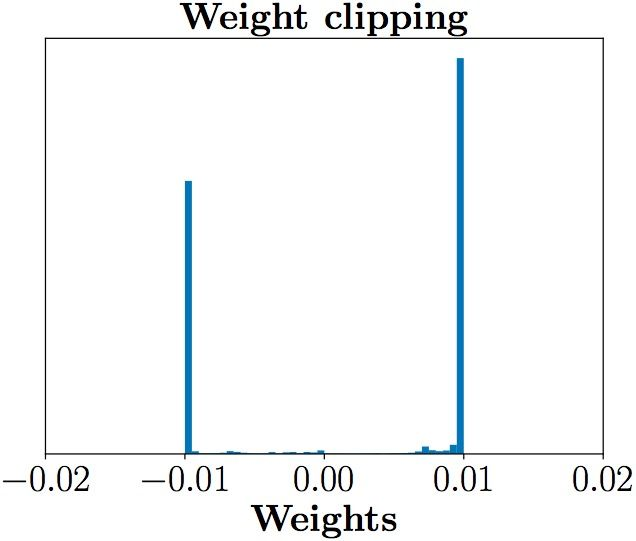
\includegraphics[width=0.45\linewidth]{figures/weight_clipping.jpg}
	\caption{Weight distribution of weight clipping}
	\label{fig:weight_clipping}
\end{figure}

This polarization will make the discriminator too weak thus leading to a bad performance. Additionally, weight clipping will lead to gradient vanishing or gradient exploding problems. Thus, the author provide an optimized method to replace weight clipping.

\subsection{Gradient penalty}

In a word, Lipschitz Continuity constrains the gradient of a function to be less than a constant $K$. So why not add this restriction into the loss function? So we modify the loss of the discriminator into the version below:

\begin{equation}
    Loss_d = E_{x \sim P_g}[D(x)]-E_{x \sim P_{data}}[D(x)]+\lambda E_{x \sim \omega}[||\nabla_x D(x)|| - K]^2
\end{equation}

where $\omega$ is the sample space and $K$ is the Lipschitz Constant which is set to be $1$ in practice. We will do sampling to approximate the three expected values in the formula in practice, but it is unreasonable to sample from the entire sample space $\omega$. As the author suggests, we can only focus on $P_g$, $P_{data}$ and the area between them. So, we define a new distribution $P_{\hat{x}}$:

\begin{equation}
    \hat{x} = \epsilon x_{data} + (1-\epsilon)x_g,\quad \epsilon \sim Uniform(0,1)
\end{equation}

Therefore, we can write down the loss of the discriminator in WGAN-GP:

\begin{equation}
    Loss_d = E_{x \sim P_g}[D(x)]-E_{x \sim P_{data}}[D(x)]+\lambda E_{x \sim P_{\hat{x}}}[||\nabla_x D(x)|| - 1]^2
\end{equation}

As a reminder, we are applying sample-independent gradient penalty, so batch normalization should not be used because it will bring in correlations between samples. So the author chooses layer normalization instead.

Because the formula above needs to compute the second gradient of the loss, some blogs propose that we can replace it with a finite difference.

\begin{equation}
    Loss_d = E_{x \sim P_g}[D(x)]-E_{x \sim P_{data}}[D(x)]+\lambda E_{x_1,x_2 \sim P_{\hat{x}}}[\frac{D(x_1)-D(x_2)}{x_1-x_2} - 1]^2
\end{equation}

Finally, for comparison, Figure \ref{fig:gradient_penalty} shows the weight distribution of gradient penalty.

\begin{figure}[h]
	\centering
	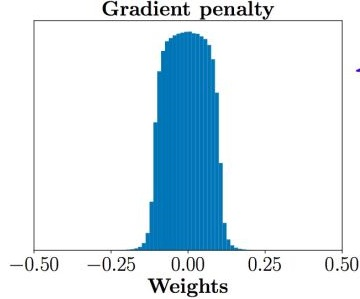
\includegraphics[width=0.45\linewidth]{figures/gradient_penalty.jpg}
	\caption{Weight distribution of gradient penalty}
	\label{fig:gradient_penalty}
\end{figure}

\section{BiGAN: Bidirection GAN}

Before all, note that there is a model called ALI, short for \emph{Adversarially Learned Inference}, it has exactly the same idea as BiGAN and both of these two papers have been recieved by ICLR 2017. But we prefer the name BiGAN. Maybe because it contains the word 'GAN'.

\subsection{Architecture of BiGAN}

In a GAN model, there are $2$ spaces: 

\begin{itemize}
    \item \textbf{the feature space} - where latent vectors $z$ are sampled from
    \item \textbf{the image space} - $P_{data}$ and $P_g$ are both sub-distributions of the image space.
\end{itemize}

\begin{figure}[h]
	\centering
	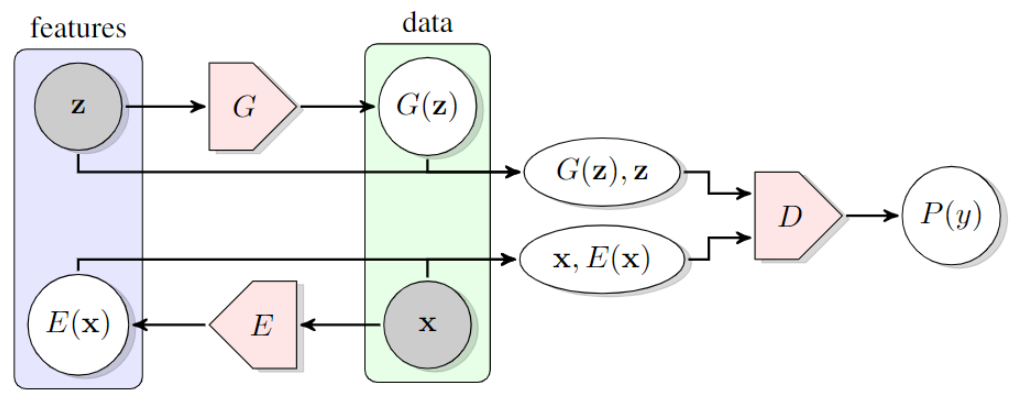
\includegraphics[width=0.8\linewidth]{figures/BiGAN.PNG}
	\caption{Architecture of BiGAN}
	\label{fig:BiGAN}
\end{figure}

As we can see in Figure \ref{fig:BiGAN}, In BiGAN, we will train a \textbf{independent} generator: an encoder that transform inputs from the \emph{image space} to the \emph{feature space} (latent space), and a decoder that transform inputs from the \emph{feature space} to the \emph{image space}. Here the bolded word \textbf{independent} means that two network will not communicate in the generator part. That is, during the training, we will not \textbf{reconstruct} an image or a latent vector to apply some similar loss like VAE.

Therefore, the encoder and decoder will only communicate in the discriminator part. The discriminator network takes inputs combined of samples from both the \emph{image space} and the \emph{feature space}. This combined input has two versions: a real sampled feature $z$ and a generated image $G(z)$, or a real sampled image $x$ and an encoded feature $E(x)$. And the discriminator aims to identify which type the combined input belongs to.

\subsection{How do G and E communicate ?}

As we known, combined inputs for the discriminator have two different types: $(G(z), z)$, or $(x, E(x))$. We can see these two types as two different distributions. The former one is the joint distribution of $P_{G(z)}$ and $P_z$. The latter one is the joint distribution of $P_x$ and $P_{E(x)}$. 

Therefore, the task of the discriminator is to decide which joint distribution the input belongs to. So the encoder $E(x)$ and the decoder $G(z)$ have to work together to fool the discriminator. The discriminator can easily make the correct answer if one of them has a bad performance.

If BiGAN finally achieves the optimal solution, two joint distributions will be exactly the same. Then the encoder and the decoder can be put together as an autoencoder to generate either reconstructed images $G(E(x))$ or reconstructed features $E(G(z))$.

The theoretical proof for these intuitions are so complex that I omit it here. Anyone interested in the proof can refer to the appendix of the original paper \href{https://arxiv.org/abs/1605.09782}{Adversarial Feature Learning}.

The BiGAN training objective is defined as a min-imax objective

\begin{equation}
    \min_{G,E} \max_{D} V(D,E,G)
\end{equation}

where

\begin{equation}
    V(D,E,G)=E_{x \sim P_{data}}[E_{z \sim P_E}[log(D(x, z))]]+E_{z \sim P_z}[E_{x \sim P_G}[log(1-D(x,z)]]
\end{equation}

\subsection{What is the difference of BiGAN and VAEGAN ?}

The idea of BiGAN and VAEGAN both comes from Autoencoder and GAN. The only difference is that in VAEGAN, the encoder and decoder will communicate in the generator part by reconstruction, but in BiGAN they will communicate in the discriminator part.

The encoder and decoder will be exactly the same if both models reach the global optimal solution. But obviously we can never achieve that in deep learning. So the actual outputs of two models will differ when we try to reconstruct an image. If we input an image of a bird. The reconstructed image from VAEGAN will still be that bird but kind of blurry. The reconstructed image from BiGAN will be sharper but maybe another bird that differ from the input one. This is the difference between VAEGAN and BiGAN.

\section{BigBiGAN: Big Bidirection GAN}

As the name suggests, BigBiGAN is a combination of BigGAN and BiGAN. Because the original BiGAN model is based on the generator proposed by DCGAN, which have relatively bad performance in image generation, thus leading to a bad performance in feature extracting. So BigBiGAN replaces the generator with BigGAN and, together with some modifications, achieves the state of are in unsupervised feature learning.

As we can see in Figure \ref{fig:BigBiGAN}, the discriminator have three parts $F$, $H$ and $J$, which respectively represent three different networks. 

The $F$ network is just like the original discriminator in traditional GAN models. It takes an image as an input and decides it is fake or not. The $H$ network, in the other hand, will distinguishes encoded latent vectors from the sampled ones. And the $J$ is similar to the discriminator in BiGAN. It will take a joint input and identify its origin - $(x, E(x))$ or $(G(z), x)$.

\begin{figure}[h]
	\centering
	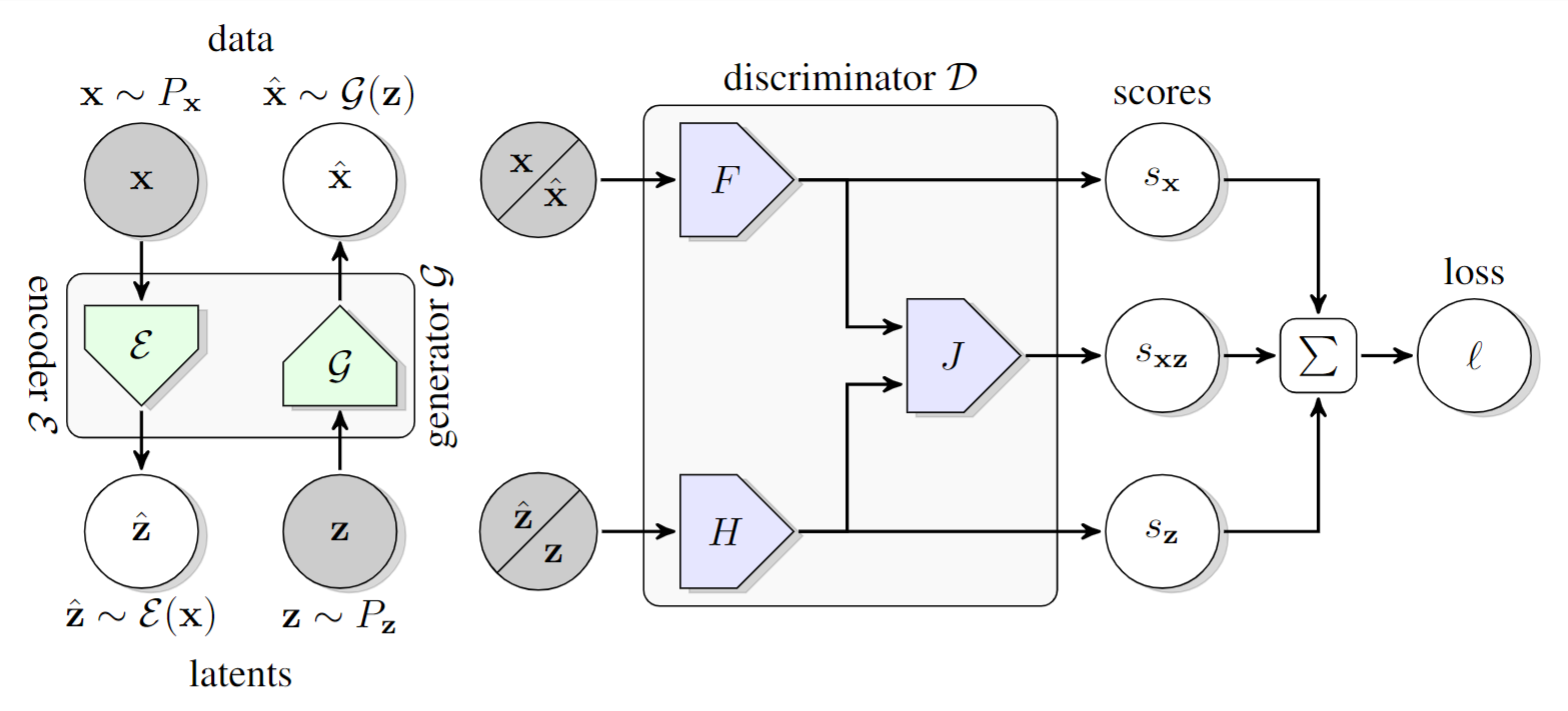
\includegraphics[width=0.8\linewidth]{figures/BigBiGAN.png}
	\caption{Architecture of BigBiGAN}
	\label{fig:BigBiGAN}
\end{figure}

All three network above will give independent scores - $s_x$, $s_z$, $s_{xz}$. The score for each sample can be computed by summing three scores up. Then we can define the loss of the generator and discriminator based on the per-sample scores:

\begin{equation}
    l_{E \& G}(x,z,y) = y(s_x + s_z + s_{xz}), \quad y \in \{-1,+1\}
\end{equation}

\begin{equation}
    Loss_{E \& G}= E_{x \sim P_{data}, \Tilde{z} \sim P_{E(x)}}[l_{E \& G}(x,\Tilde{z},+1)] + E_{z \sim P_z, \Tilde{x} \sim P_{G(z)}}[-l_{E \& G}(\Tilde{x},z,-1)]
\end{equation}

\begin{equation}
    l_D(x,z,y)=h(y \times s_x)+h(y \times s_z)+h(y \times s_{xz}), \quad y \in \{-1,+1\}
\end{equation}

\begin{equation}
    Loss_D=E_{x \sim P_{data}, \Tilde{z} \sim P_{E(x)}}[l_D(x,\Tilde{z},+1)] + E_{z \sim P_z, \Tilde{x} \sim P_{G(z)}}[-l_D(\Tilde{x},z,-1)]
\end{equation}

where $h(t)=\max (0,1-t)$ is a hinge function used to regularize the discriminator, also used in BigGAN. Then other architecture details are the same as it is in BiGAN or BigGAN. Together with some training techniques like \emph{truncation tricks}, the performance of BigBiGAN is surprising. It does not only defeat BigGAN in image generation, but also outperforms those unsupervised representation learning algorithms on ImageNet.

That is all for BigBiGAN. \textbf{Bigger}, \textbf{larger}, and \textbf{stronger}.

\section{Summary of GAN zoo}

\subsection{InfoGAN: Information GAN}

As shown in Figure \ref{fig:InfoGAN}, InfoGAN will first separate the latent vector into two part $c$ and $z^{'}$. Part $c$ is expected to contain the encoded information of the generated images $x$ and $z^{'}$ represents the variant part which can not be learned during the training. 

\begin{figure}[h]
	\centering
	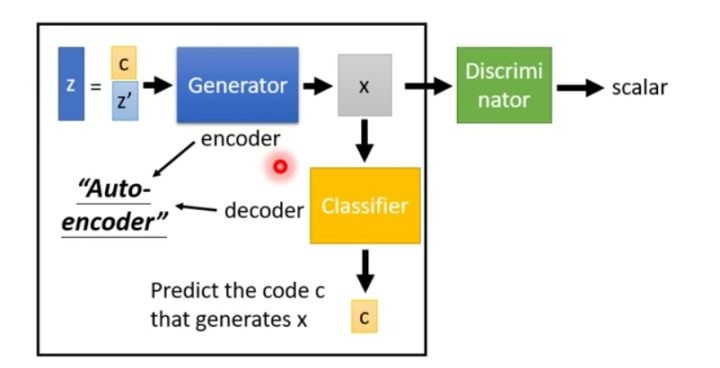
\includegraphics[width=0.6\linewidth]{figures/InfoGAN.jpg}
	\caption{Architecture of InfoGAN}
	\label{fig:InfoGAN}
\end{figure}

The generator, acting as an inverse encoder, will transform the $c+z^{'}$ vector into an image $x$. A additional classifier network, acting as an inverse decoder, will predict the code $c$ that generates $x$. Also a discriminator network is necessary for the model to generate a realistic image instead of an image that is easy to predict $c$ but totally unrealistic.

\subsection{SAGAN: Self-Attension GAN}

Since GAN models use transposed convolutions to scan feature maps, they only have access to nearby information. But when painting a picture, we should focus on the overall layout of the image instead of only looking at the local parts. SAGAN tries to handle this problem.

\textbf{Attention} is a useful technique that can be apply to various specific deep learning areas and GAN is one of them. As a brief summary, an attention will have three matrices \textbf{Q}uery, \textbf{K}ey and \textbf{V}alue. And the query and key decide how much the value can speak to the outer world (shown in Figure \ref{fig:Attention}). When it comes to \textbf{self-attention}, it means that the query, key and value are all same.

\begin{figure}[h]
	\centering
	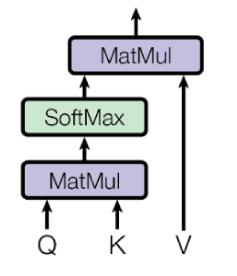
\includegraphics[width=0.2\linewidth]{figures/Attention.png}
	\caption{Attention}
	\label{fig:Attention}
\end{figure}

We will apply self-attention to every layer of both generator and discriminator network. Figure \ref{fig:Architecture_SAGAN} shows the architecture of SAGAN. And the construction of the attention map is shown in Figure \ref{fig:Attention_map_SAGAN}. By combining the self-attention part, SAGAN can take care of the overall layout of the image and generate more realistic images.

\begin{figure}[h]
	\centering
	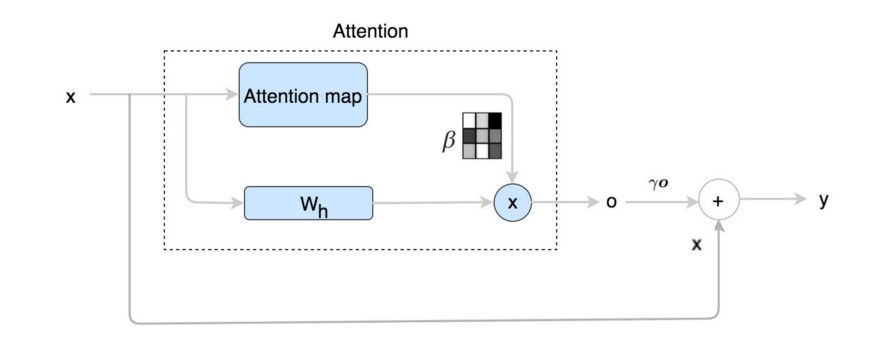
\includegraphics[width=0.7\linewidth]{figures/SAGAN_layer.jpeg}
	\caption{Architecture of SAGAN}
	\label{fig:Architecture_SAGAN}
\end{figure} 

\begin{figure}[h]
	\centering
	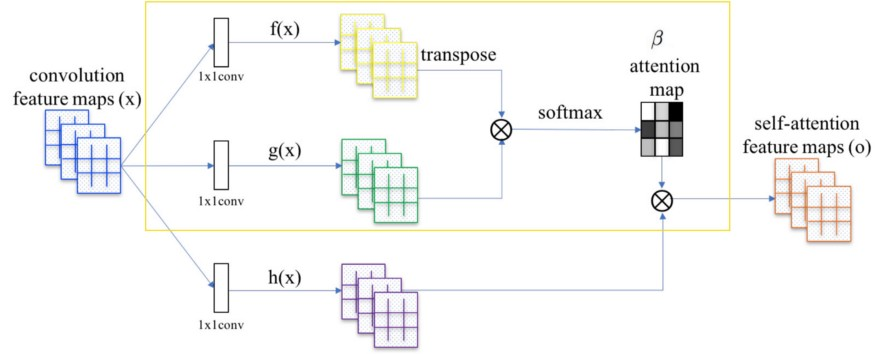
\includegraphics[width=0.7\linewidth]{figures/SAGAN_Attentino_map.jpeg}
	\caption{Attention map of SAGAN}
	\label{fig:Attention_map_SAGAN}
\end{figure}

\subsection{VAEGAN: Variational Autoencoder GAN}

As shown in Figure \ref{fig:VAEGAN}, VAEGAN combines VAE and GAN. The real images sampled from $P_{data}$ will first be put into an encoder to produce a latent vector $z$. Then the generator, acting as a decoder, will decode the latent vector $z$ to generate a reconstructed image $\Tilde{}{x}$. Next, the discriminator aims to distinguish the reconstructed images $\Tilde{x}$ from the real images $x$.

\begin{figure}[h]
	\centering
	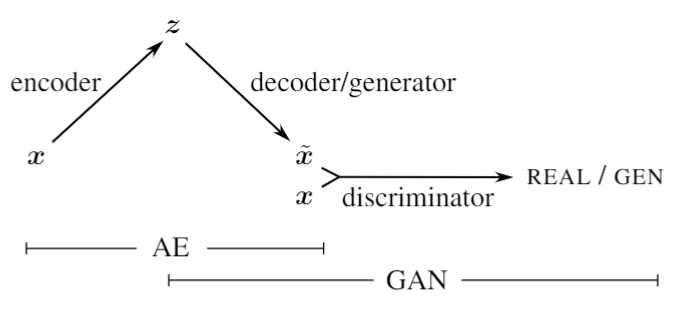
\includegraphics[width=0.7\linewidth]{figures/VAEGAN.PNG}
	\caption{Architecture of VAEGAN}
	\label{fig:VAEGAN}
\end{figure}

\section{Work next week}

I think I have gone through most of the important GAN models since $2014$ (except BigGAN). Next I will focus on implementing and fine-tuning GAN models. 

Besides, I have arranged my paper notes in one pdf file. But I do not think they are in a good order and shape. I wonder if there is some recommendations for organizing paper notes for future referring.

\end{document}